\documentclass{beamer}
\usetheme{AnnArbor}
\usecolortheme{spruce}
\usepackage{circuitikz}
\usepackage{graphicx}

\title{Multipliers, Iterative Algorithms, Negative Numbers}
\subtitle{Leveraging Adders for a Greater Purpose}
\author[A Praveen \& A Krishnan]{Akilesh Praveen \& Ashwath Krishnan}
\institute{UMD}
\date{\today}



\begin{document}

    % title page
    \begin{frame}
        \titlepage
    \end{frame}
    
    % table of contents
    \begin{frame}
        \frametitle{Agenda}
        \tableofcontents
    \end{frame}
    
    \section{Announcements}
    
        \begin{frame}
                \vfill
                \centering
                \begin{beamercolorbox}[sep=8pt,center,shadow=true,rounded=true]{title}
                    \usebeamerfont{title}Announcements\par%
                \end{beamercolorbox}
                \vfill
             \end{frame}
    
        \subsection{Project 3}
        
            
            
            \begin{frame}
                \frametitle{Project 3}
                \begin{itemize}
                    \item Project 3's been released, and the name of the game is multipliers.
                    \item You'll find everything you need under the 'week 4' section on the course website
                    \item Today's lecture will give you all the background knowledge that you need to know about implementing a multiplier
                    
                    \item More info to come at the end of lecture
                    
                \end{itemize}
            \end{frame}
            
            \begin{frame}
            	\frametitle{Some Reminders}
            	\begin{itemize}
            		\item As the projects become more involved, we'd like to remind you to reach out and attend office hours if you are struggling.
                    \item Additionally, here's a reminder that all projects can be group projects, but you'll have to let us know \textbf{4 days} prior to the project's due date if you'll be working in a group. (Max size of 3)
            	\end{itemize}
            	
            \end{frame}
        
    \section{Multipliers}
    
    	\begin{frame}
                \vfill
                \centering
                \begin{beamercolorbox}[sep=8pt,center,shadow=true,rounded=true]{title}
                    \usebeamerfont{title}Multipliers\par%
                \end{beamercolorbox}
                \vfill
             \end{frame}
    
    	\subsection{Multiplication in Binary}
    
    	\begin{frame}
    		\frametitle{A Question}
    		\begin{center}
    			{\Large How does multiplication work in binary?}
    		\end{center}
    	\end{frame}
    	
    	\begin{frame}
    		\frametitle{Multiplication Table}
    		\begin{itemize}
    			\item Multiplication works the same way in binary as it does in base-10!
    			\item Just like single digit multiplication in base-10 goes up to $ 9 \times 9 $, single digit multiplication in binary goes up to $ 1 \times 1$
    			\item Here's the basic multiplication table for binary:

    		\end{itemize}
    		
    		\centering
    		{\Large
    		\begin{tabular}{ |c|c|c| }
					\hline
				 	 & \textbf{0} & \textbf{1} \\ 
				 	\hline
				 	\textbf{0} & 0 & 0 \\  
				 	\hline
				 	\textbf{1} & 0 & 1 \\
				 	\hline 
					\end{tabular}
					}
    	\end{frame}
    	
    	\begin{frame}
    		\frametitle{Multiplication}
    		\begin{itemize}
    			\item Before you get very excited, this is only a small bit of what we're after.
    			\item Now, we know how to multiply one-bit numbers (Yay!)
    			\begin{itemize}
    				\item note that \texttt{AND} is all you need to represent this operation
    			\end{itemize}
    			\item In binary, multiplication is the same as it's always been for us in decimal
    			\item Let's go through an example now
    		\end{itemize}
    	\end{frame}
    	
    	
    	\begin{frame}
    		\frametitle{Multiplication}
    		
    		\begin{itemize}
    			\item Again, we will look to the 'long' way of doing this computation for inspiration
    		\end{itemize}

			\centering    		
    		
    		{\Huge
			\begin{tabular}{c@{\,}c@{\,}c@{\,}c@{\,}c@{\,}c@{\,}c@{\,}c@{\,}c@{\,}c}
					   & &  &  &  &  & 1 & 1 & 0 & 1 \\
					   & &  &  &  & $\times$ & 1 & 0 & 1 & 1 \\
					   \hline
					   
					
					
			\end{tabular}}
			\vfill
    	\end{frame}
    	
    	
    	\begin{frame}
    		\frametitle{Multiplication}

			\centering    		
    		
    		{\Huge
			\begin{tabular}{c@{\,}c@{\,}c@{\,}c@{\,}c@{\,}c@{\,}c@{\,}c@{\,}c@{\,}c}
					   & &  &  &  &  & 1 & 1 & 0 & 1 \\
					   & &  &  &  & $\times$ & 1 & 0 & 1 & 1 \\
					   \hline
					   & &  &  &  &   & 1 & 1 & 0 & 1 \\
					   & &  &  &  & 1 & 1 & 0 & 1 & {\color{red}0} \\
					   & &  &  & 0 & 0 & 0 & 0 & {\color{red}0} & {\color{red}0} \\
					   & &  & 1 & 0 & 1 & 1 & {\color{red}0} & {\color{red}0} & {\color{red}0} \\
					   \hline
					    &  & 1 & 0 & 0 & 0 & 1 & 1 & 1 & 1
					
					
			\end{tabular}}
			\vfill
    	\end{frame}
    	
    	
    	\begin{frame}
    		\frametitle{What can we gather?}
    		\begin{itemize}
    			\item What exactly can we gather from doing this computation out longhand?
    			\begin{itemize}
    				\item Binary multiplication is even easier than decimal; we only have two choices: 1 or 0
    				\item Go from right to left, multiplying out the individual numbers
    				\item After some analysis, this appears to be repeated additions (which are somewhat similar each time)
    				\item We will implement multiplication the same way!
    				\item By leveraging repeated sets of Full Adders, we can easily perform these repeated additions.
    			\end{itemize}
    			\item Q: But Aki, what if we have too many carries in a single column for a FA to add???
    			\begin{itemize}
    				\item A: We're screwed
    			\end{itemize}
    		\end{itemize}
    	\end{frame}
    	
    	\begin{frame}
    		
    			\frametitle{Partial Additions}
    			\begin{itemize}
    				\item Remember how some columns had us adding more than the maximum that a Full Adder could handle? 
    				\begin{itemize}
    					\item Let's try and address that
					\end{itemize}
    				\item In other words, we want to cut down this big computation into chunks juust small enough so that Full Adders can handle each chunk of it
    				\item Formally, this sort of black magic is called 'Partial Additions'- look to the whiteboard for a demonstration
    				\begin{itemize}
    					\item I've also got a video up on the course website explaining this stuff in more detail if you want more clarification
    				\end{itemize}
    			\end{itemize}
    		
    	\end{frame}
    	
    	\begin{frame}
    		\frametitle{Bringing it all Together}
    		\begin{itemize}
    			\item We know how to multiply one-bit numbers
    			\item We know how to add said numbers together with Full Adders
    			\item We've come up with a clever way to make sure we don't have more carries than we can handle
    			\item Now we just need to implement it (and repeat it a bunch!)
    		\end{itemize}
    	\end{frame}
    	
    	\begin{frame}
    		\frametitle{The Actual Circuit}
    		\centering
    		
\includegraphics[width=0.85\textwidth]{comb_multiplier}
    	\end{frame}
    	
    	\begin{frame}
    		\frametitle{Some Additional Notes}
    		\begin{itemize}
    			\item This is what we call a \textbf{combinatorial multiplier}.
    			\item There are other ways to implement multipliers
    		\end{itemize}
    	\end{frame}
    	
    	

		\subsection{Limitations}    	
    	
		\begin{frame}
    		\frametitle{Multiplication with Negatives}
    		\begin{itemize}
    			\item What if we want to multiply negative numbers?
    			\item We're going to use the standard 'Two's Complement', but with a special twist for our application.
    			
    		\end{itemize}
    	\end{frame}
    	
    	\begin{frame}
    		\frametitle{Two's Complement}
    		\begin{itemize}
    			\item Say we wanted to represent the number \textbf{5} as a negative number.
    			\item First, let's write it binary
    			\begin{itemize}
    				\item \texttt{0101}
    			\end{itemize}
    			\item Next, let's flip all the bits
    			\begin{itemize}
    				\item \texttt{1010}
    			\end{itemize}
    			\item Finally, let's add 1
    			\begin{itemize}
    				\item \texttt{1011}
    			\end{itemize}
    			
    			\item It turns out, this isn't all we need. There's one more nuance to using Two's Complement with multiplication.
    			
    		\end{itemize}
    	\end{frame}  
    	
    	\begin{frame}
    		\frametitle Two's Complement
    		\begin{itemize}
    			\item We will need to extend our multiplier and multiplicand before multiplying
    			\item This is because carries are \textbf{POSSIBLE} all the way up till the leftmost most significant bit
    			\item Think of these leading 1's as 'insurance' bits to make sure that Two's Complement kicks in. (Carries will ruin the two's complement business we've got going)
    			\item Think of it this way: both \texttt{11} and \texttt{1111111111} are both Two's Complement representations of -1
    		\end{itemize}
    	\end{frame}
    	
    	\begin{frame}
    		\frametitle{Two's Complement}
    		\centering
    		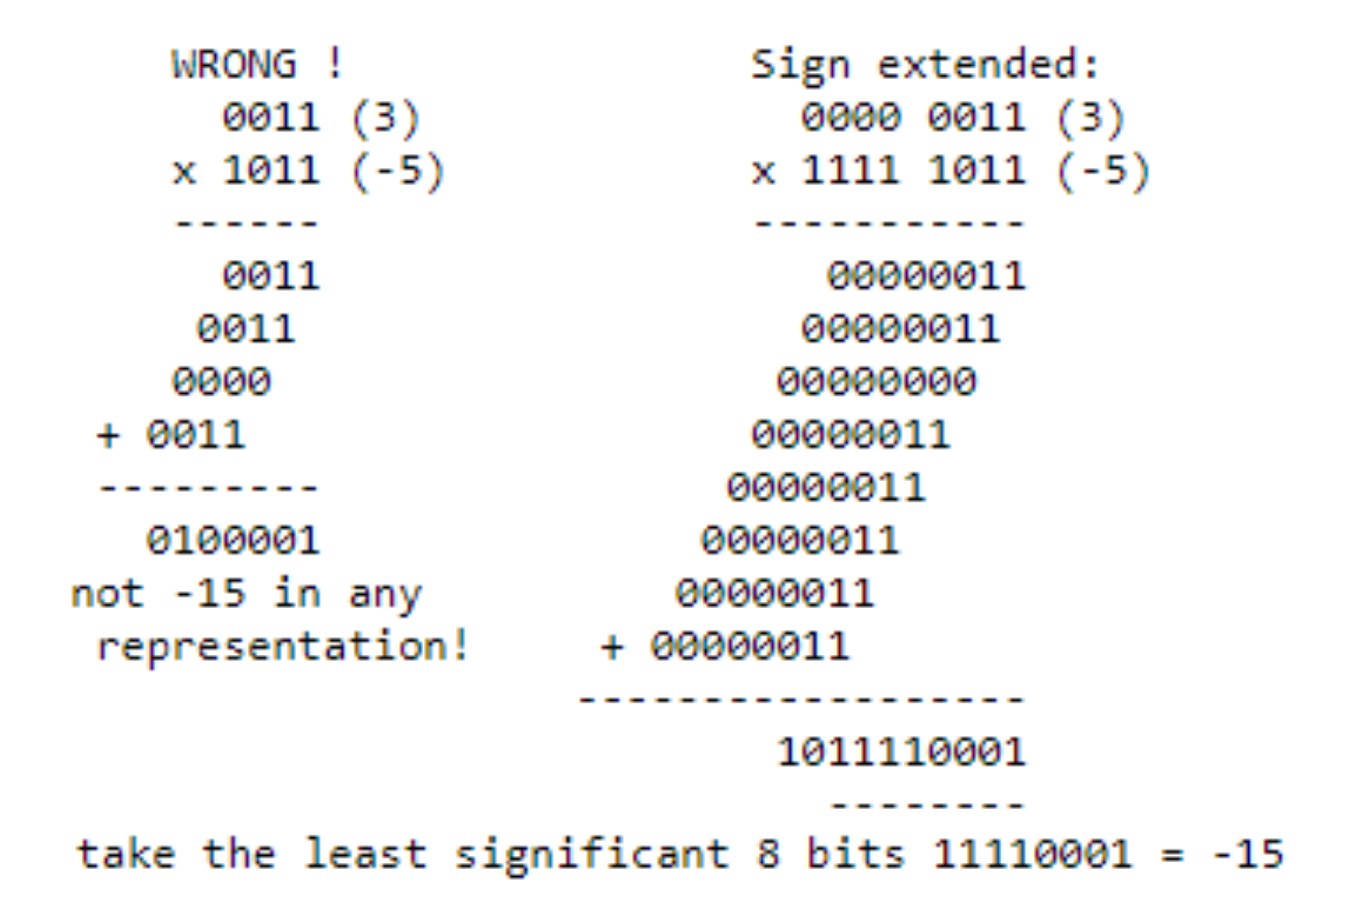
\includegraphics[width=0.85\textwidth]{multiplier}
    	\end{frame}    	   	
    	
    	
    	\begin{frame}
    		\frametitle{Limitations}
    		\begin{itemize}
    			\item Addition, Subtraction (check out the two's complement video on the course website), and Multiplication- we've done it all.
    			\item What about division? Exponentiation?
    			\item The Answer: \textbf{It's harder}
    			\item One Solution: Iterative algorithms
    		\end{itemize}
    	\end{frame}
    	
    	
    	
		\section{Iterative Algorithms}    	
    	
    	\begin{frame}
                \vfill
                \centering
                \begin{beamercolorbox}[sep=8pt,center,shadow=true,rounded=true]{title}
                    \usebeamerfont{title}Iterative Algorithms\par%
                \end{beamercolorbox}
                \vfill
             \end{frame}
             
    	
    	\subsection{Iterative Algorithms}
    	
    	\begin{frame}
    		\frametitle{Iterative Algorithms}
    		\begin{itemize}
    			\item Why would we want to use this fancy sounding method?
    			\item Reusing adders will help us- saving gates at the cost of speed
    			\item This is where we begin bridging the gap between the cave-person computer science we're doing and what's actually in computers these days
    		\end{itemize}
    	\end{frame}
    	
    	\begin{frame}
    		\frametitle{Division}
    		\begin{itemize}
    			\item Consider division for a moment- how would we do a classic division?
    			\begin{itemize}
    				\item No, I'm not whipping out some long division example for you guys
    				\item Q: Is it possible to convert this to binary, though?
    				\item A: We can try!
    			\end{itemize}
    			\item Additionally, now that we know how multiplication works, we can also explore the next stage! Exponentiation!
    			\begin{itemize}
    				\item Think about how you'd use iterative algorithms and what we've already learned about multiplication in order to efficiently accomplish. (It's a little more than just a few stacked adders)
    			\end{itemize}
    		\end{itemize}
    	\end{frame}
    	
    	
    	\begin{frame}
    		\frametitle{Division \& Exponentiation}
    		\begin{itemize}
    			\item This is a 1-credit class, so we won't be going over this in lecture. More on division and exponentiation will be posted online, but don't expect it on the exam. (It's fun stuff, though!)
    		\end{itemize}
    	\end{frame}
    	
    	
    	
    	% TODO Finish section on iterative division algorithm
    	% TODO Mention 2's complement application will be online
    	% TODO Talk about the project
    	
    	
    \section{Project 3}
    
    	\begin{frame}
                \vfill
                \centering
                \begin{beamercolorbox}[sep=8pt,center,shadow=true,rounded=true]{title}
                    \usebeamerfont{title}Project 3\par%
                \end{beamercolorbox}
                \vfill
             \end{frame}
   
    
\end{document}
